This section provides a comprehensive overview of the evaluation criteria, results, and analysis for both the Logistic Regression and LSTM-based neural network models, along with observations from the chatbot usage. By detailing the different conditions and their corresponding metrics, the analysis highlights the improvements achieved with the LSTM model and provides insights into the model's performance under various configurations.

\subsection{Evaluation Criteria}
Based on the study by Katsumata(2020)\cite{Katsumata}, I used these metrics to evaluate the performance of the spell-correcting chatbot:
\begin{itemize}
    \item \textbf{Accuracy}: The proportion of correctly identified instances (correct or misspelled) out of the total instances.
    \item \textbf{Precision}: The ratio of correctly predicted positive observations to the total predicted positives.
    \item \textbf{Recall}: The ratio of correctly predicted positive observations to all observations in the actual class.
    \item \textbf{F1 Score}: The weighted average of Precision and Recall, providing a balance between the two.
\end{itemize}

These metrics provide a comprehensive evaluation of the models' performance, considering both their ability to correctly identify misspellings and their reliability in predicting the correct class.

\subsection{Logistic Regression Model}

I experimented with the Logistic Regression model using three different error rates for introducing misspellings: 10\%, 50\%, and 80\%. Regardless of the error rate, the results were consistent across all trials.

\subsubsection{Logistic Regression Model Results}

\begin{verbatim}
Accuracy: 0.4645
             precision  recall  f1-score   support

           0      0.47    0.65    0.55     47305
           1      0.44    0.28    0.35     47390

    accuracy                      0.46     94695
   macro avg      0.46    0.46    0.45     94695
weighted avg      0.46    0.46    0.45     94695
\end{verbatim}

\begin{figure}[h!]
    \centering
    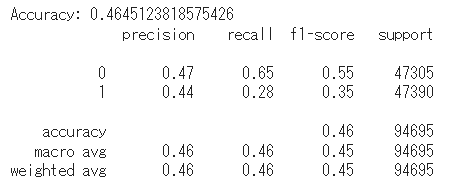
\includegraphics[width=0.3\textwidth]{LogiReg_result.png}
    \caption{Evaluation results of Logistic Regression model.}
    \label{fig:logreg_results}
\end{figure}

\subsection{LSTM-Based Neural Network Model}

To optimize and improve accuracy, I built an LSTM-based neural network model. I experimented with various combinations of error rates, epochs, and batch sizes:

\begin{itemize}
    \item \textbf{(error rate = 0.1, epochs = 10, batch size = 64)}
    \item \textbf{(error rate = 0.5, epochs = 10, batch size = 64)}
    \item \textbf{(error rate = 0.5, epochs = 10, batch size = 32)}
    \item \textbf{(error rate = 0.8, epochs = 10, batch size = 64)}
\end{itemize}

\subsubsection{LSTM Model Results}

1. \textbf{(error rate = 0.1, epochs = 10, batch size = 64)}
\begin{verbatim}
Accuracy: 0.5153
             precision  recall  f1-score   support

           0      0.51     0.76     0.61     47305
           1      0.53     0.27     0.36     47390

    accuracy                        0.52     94695
   macro avg      0.52     0.52     0.48     94695
weighted avg      0.52     0.52     0.48     94695
\end{verbatim}

\begin{figure}[h!]
    \centering
    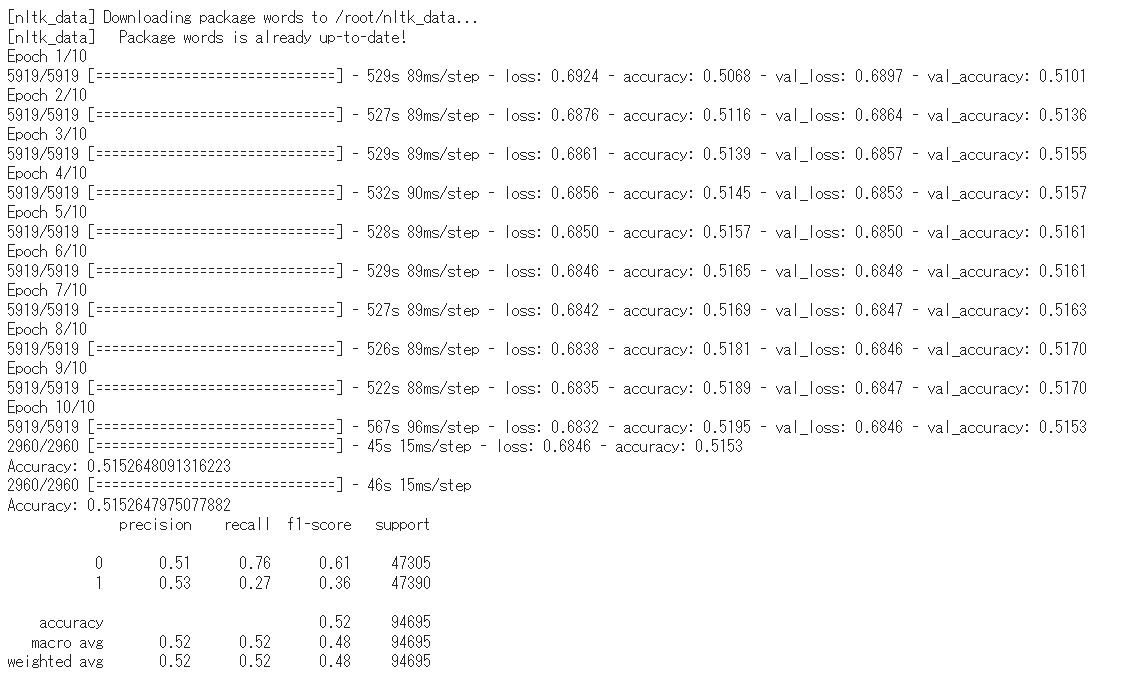
\includegraphics[width=0.3\textwidth]{ER10_epoch10_batch64.png}
    \caption{Evaluation results of LSTM model with error rate 0.1, epochs 10, batch size 64.}
    \label{fig:lstm_results_0.1_10_64}
\end{figure}

2. \textbf{(error rate = 0.5, epochs = 10, batch size = 64)}
\begin{verbatim}
Accuracy: 0.6380
            precision    recall  f1-score   support

           0      0.59     0.91     0.71    47305
           1      0.80     0.37     0.50    47390

    accuracy                        0.64     94695
   macro avg      0.69     0.64     0.61     94695
weighted avg      0.69     0.64     0.61     94695
\end{verbatim}

\begin{figure}[h!]
    \centering
    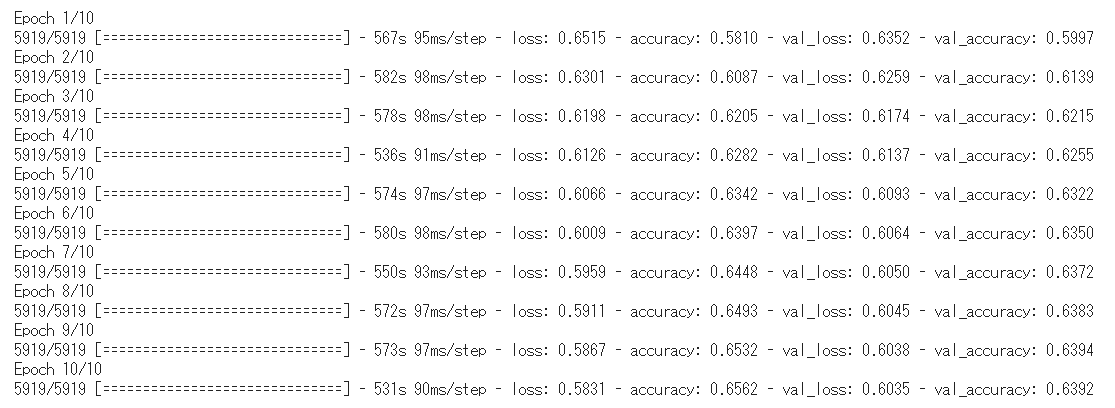
\includegraphics[width=0.3\textwidth]{1-ER50_epoch10_batch64.png}
    \label{fig:lstm_results_0.5_10_64-1}
\end{figure}
\begin{figure}[h!]
    \centering
    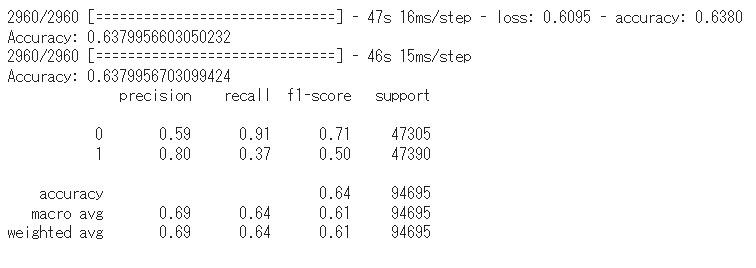
\includegraphics[width=0.3\textwidth]{2-ER50_epoch10_batch64.png}
    \caption{Evaluation results of LSTM model with error rate 0.5, epochs 10, batch size 64.}
    \label{fig:lstm_results_0.5_10_64-2}
\end{figure}

3. \textbf{(error rate = 0.5, epochs = 10, batch size = 32)}
\begin{verbatim}
Accuracy: 0.6408
            precision    recall  f1-score   support

           0      0.59     0.91    0.72    47305
           1      0.81     0.37    0.51    47390

    accuracy                       0.64     94695
   macro avg      0.70     0.64    0.61     94695
weighted avg      0.70     0.64    0.61     94695
\end{verbatim}

\begin{figure}[h!]
    \centering
    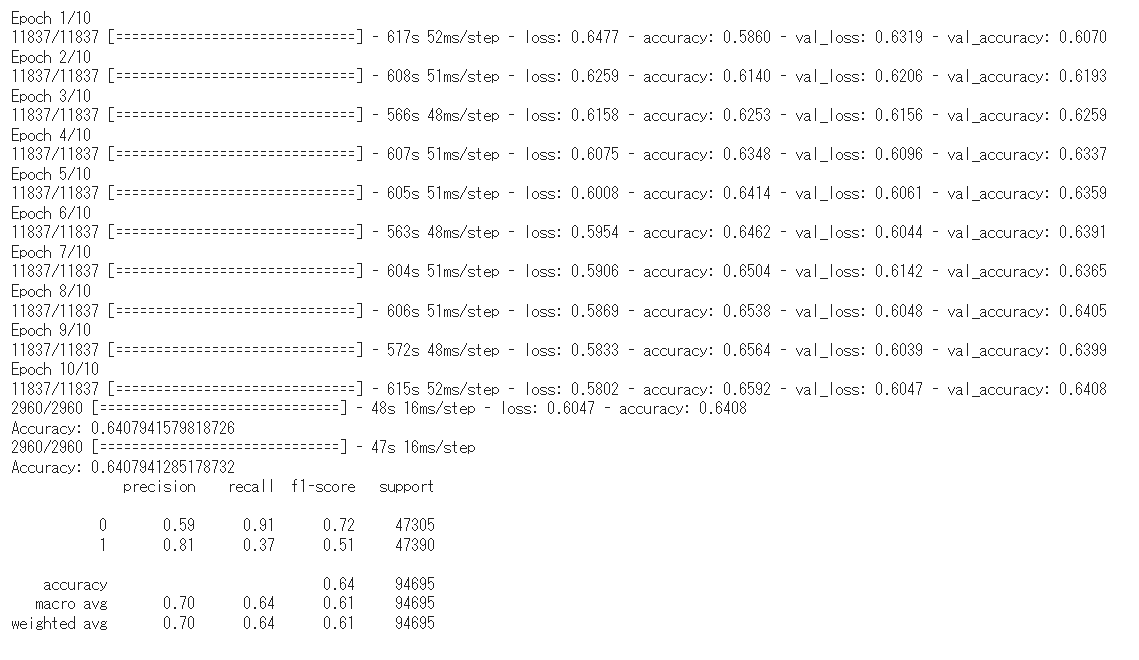
\includegraphics[width=0.3\textwidth]{ER50_epoch10_batch32.png}
    \caption{Evaluation results of LSTM model with error rate 0.5, epochs 10, batch size 32.}
    \label{fig:lstm_results_0.5_10_32}
\end{figure}

4. \textbf{(error rate = 0.8, epochs = 10, batch size = 64)}
\begin{verbatim}
Accuracy: 0.7451
            precision    recall  f1-score   support

           0      0.69     0.89     0.78    47305
           1      0.84     0.60     0.70    47390

    accuracy                        0.75    94695
   macro avg      0.77     0.75     0.74    94695
weighted avg      0.77     0.75     0.74    94695
\end{verbatim}

\begin{figure}[h!]
    \centering
    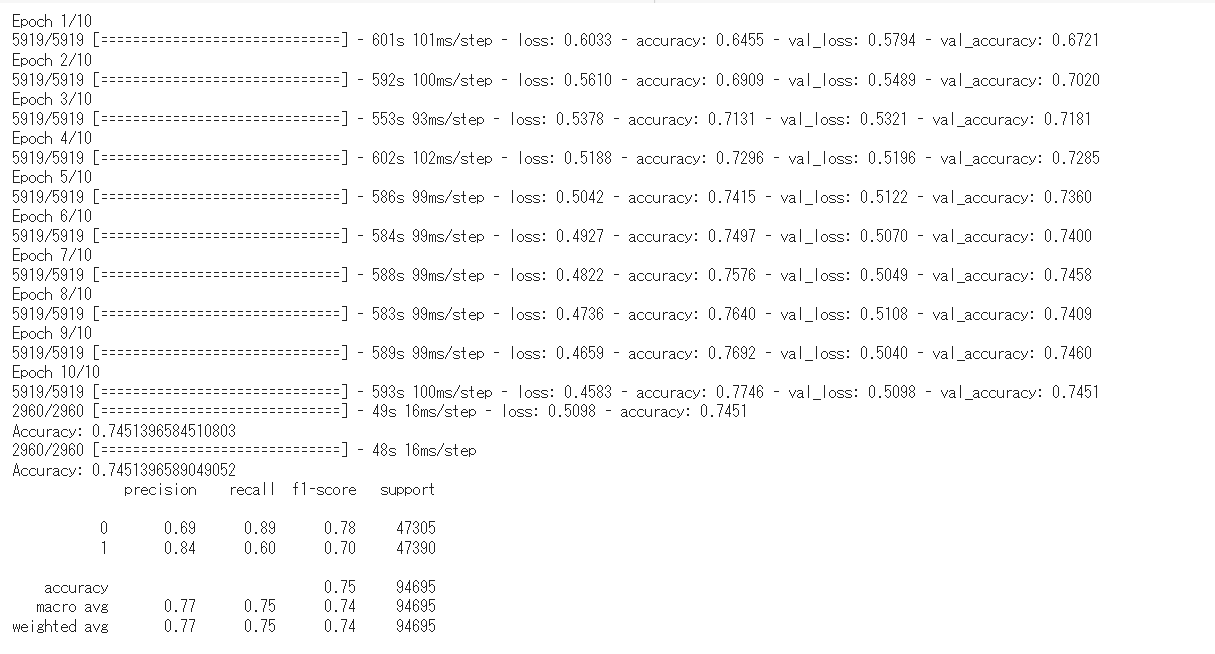
\includegraphics[width=0.3\textwidth]{ER80_epoch10_batch64.png}
    \caption{Evaluation results of LSTM model with error rate 0.8, epochs 10, batch size 64.}
    \label{fig:lstm_results_0.8_10_64}
\end{figure}

\subsection{Analysis}

\subsubsection{Logistic Regression Model}

The Logistic Regression model achieved an accuracy of approximately 46.45\%, with a precision of 0.47 for class 0 (correct words) and 0.44 for class 1 (misspelled words). The recall for class 0 was higher (0.65) compared to class 1 (0.28), indicating that the model was better at identifying correctly spelled words than misspelled ones. The F1 score, a balance between precision and recall, was moderate for class 0 (0.55) and lower for class 1 (0.35).

Overall, the Logistic Regression model provided a baseline performance but lacked the capability to accurately detect and correct misspelled words, regardless of the error rate used.

\subsubsection{LSTM-Based Neural Network Model}

The LSTM model showed significant improvement over the Logistic Regression model, with varying results based on the error rate and batch size:

1. \textbf{(error rate = 0.1, epochs = 10, batch size = 64)}: Accuracy was 51.53\%, with better performance for class 0 (precision: 0.51, recall: 0.76) compared to class 1 (precision: 0.53, recall: 0.27).

2. \textbf{(error rate = 0.5, epochs = 10, batch size = 64)}: Accuracy increased to 63.80\%, with notable improvements in class 1 detection (precision: 0.80, recall: 0.37).

3. \textbf{(error rate = 0.5, epochs = 10, batch size = 32)}: Slightly better accuracy at 64.08\%, with similar performance metrics as the previous configuration.

4. \textbf{(error rate = 0.8, epochs = 10, batch size = 64)}: The highest accuracy achieved was 74.51\%, with significant improvements in both precision and recall for class 1 (precision: 0.84, recall: 0.60).

These results indicate that the LSTM model is more effective at handling higher error rates, showing robust performance in detecting and correcting misspelled words. The choice of batch size also played a role, with smaller batch sizes slightly improving accuracy and F1 scores.

\subsection{Observations from Chatbot Usage}

Despite the improved metrics with the LSTM model, the real-world usage of the chatbot revealed that the suggestion accuracy was quite low. This discrepancy highlights a common challenge in NLP and machine learning: metrics may not fully capture the practical effectiveness of a model. User experience can often expose limitations that quantitative evaluations might overlook.

\begin{figure}[h!]
    \centering
    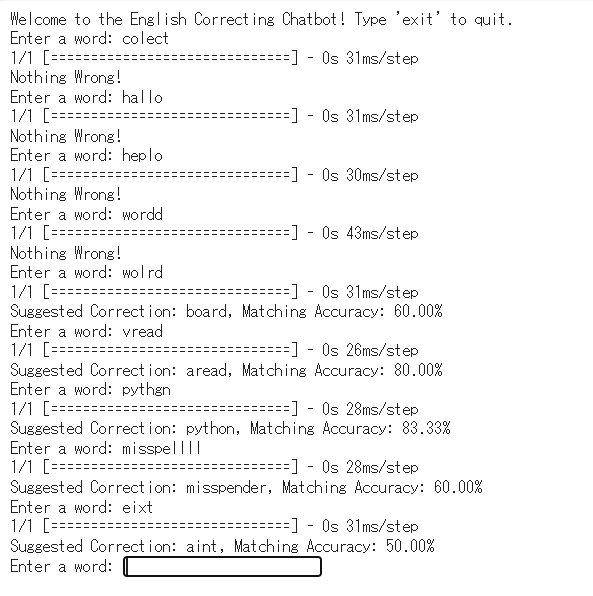
\includegraphics[width=0.3\textwidth]{chatbot_display.png}
    \caption{Example Chatbot Usage.}
    \label{fig:lchatbot_display}
\end{figure}